%preamble
\documentclass[letterpaper]{article}
\synctex=1
\usepackage{graphicx}
\graphicspath{ {images/} }

\usepackage{lipsum}
\usepackage{float}

\usepackage{amssymb}

\usepackage{siunitx}

\usepackage{multirow}
% for merging table cells I think

\usepackage{tabularx}
% allows for linewrap within cells
\newcolumntype{Y}{>{\centering\arraybackslash}X}

\usepackage{todonotes}
\usepackage{hyperref}

\usepackage{pdfpages} % for attaching the table lol




\title{ECE 322 \\
Lab Reporrt 1}
\author{Arun Woosaree\\
XXXXXXX}
\begin{document}
 \maketitle 

 \section*{Introduction}
 The purpose of this lab was to serve as a practical introduction to rudimentary black-box testing techniques.
 The testing methods introduced were dirty testing, error guessing, and partition-based testing.
 It should be noted that numerous other black-box testing methods exist
 The idea of black-box testing is that tests are carried out with no knowledge of how the software
 internally works. In other words, the implementation details are a ``black box'' as the name would suggest.

\section*{Part 1 - Failure/Dirty Testing, Error Guessing}
For task one in this lab, we had to be creative, as is the nature of Failure/Dirty testing, and error guessing.
The purpose was to test the functionality of a calculator program.

\section*{Part 2 - Partition Testing}

\subsection*{Triangle Equivalence Classes}
\subsubsection*{Valid}
\begin{enumerate}
    \item $a + b > c$
    \item Equilateral
    \item Isoscoles
    \item Scalene
    \item 3 arguments
    \item separated by one space
    \item positive integers
\end{enumerate}

\subsubsection*{Invalid}
\begin{enumerate}
    \item $a + b = c$
    \item $ a + b < c$
    \item $< 3$ arguments
    \item $> 3$ arguments
    \item separated by more than one space
    \item negative argument
    \item argument with the number `0'
    \item decimal argument
\end{enumerate}





\section*{Appendix}
\appendix
\section{Calculator Test Cases}
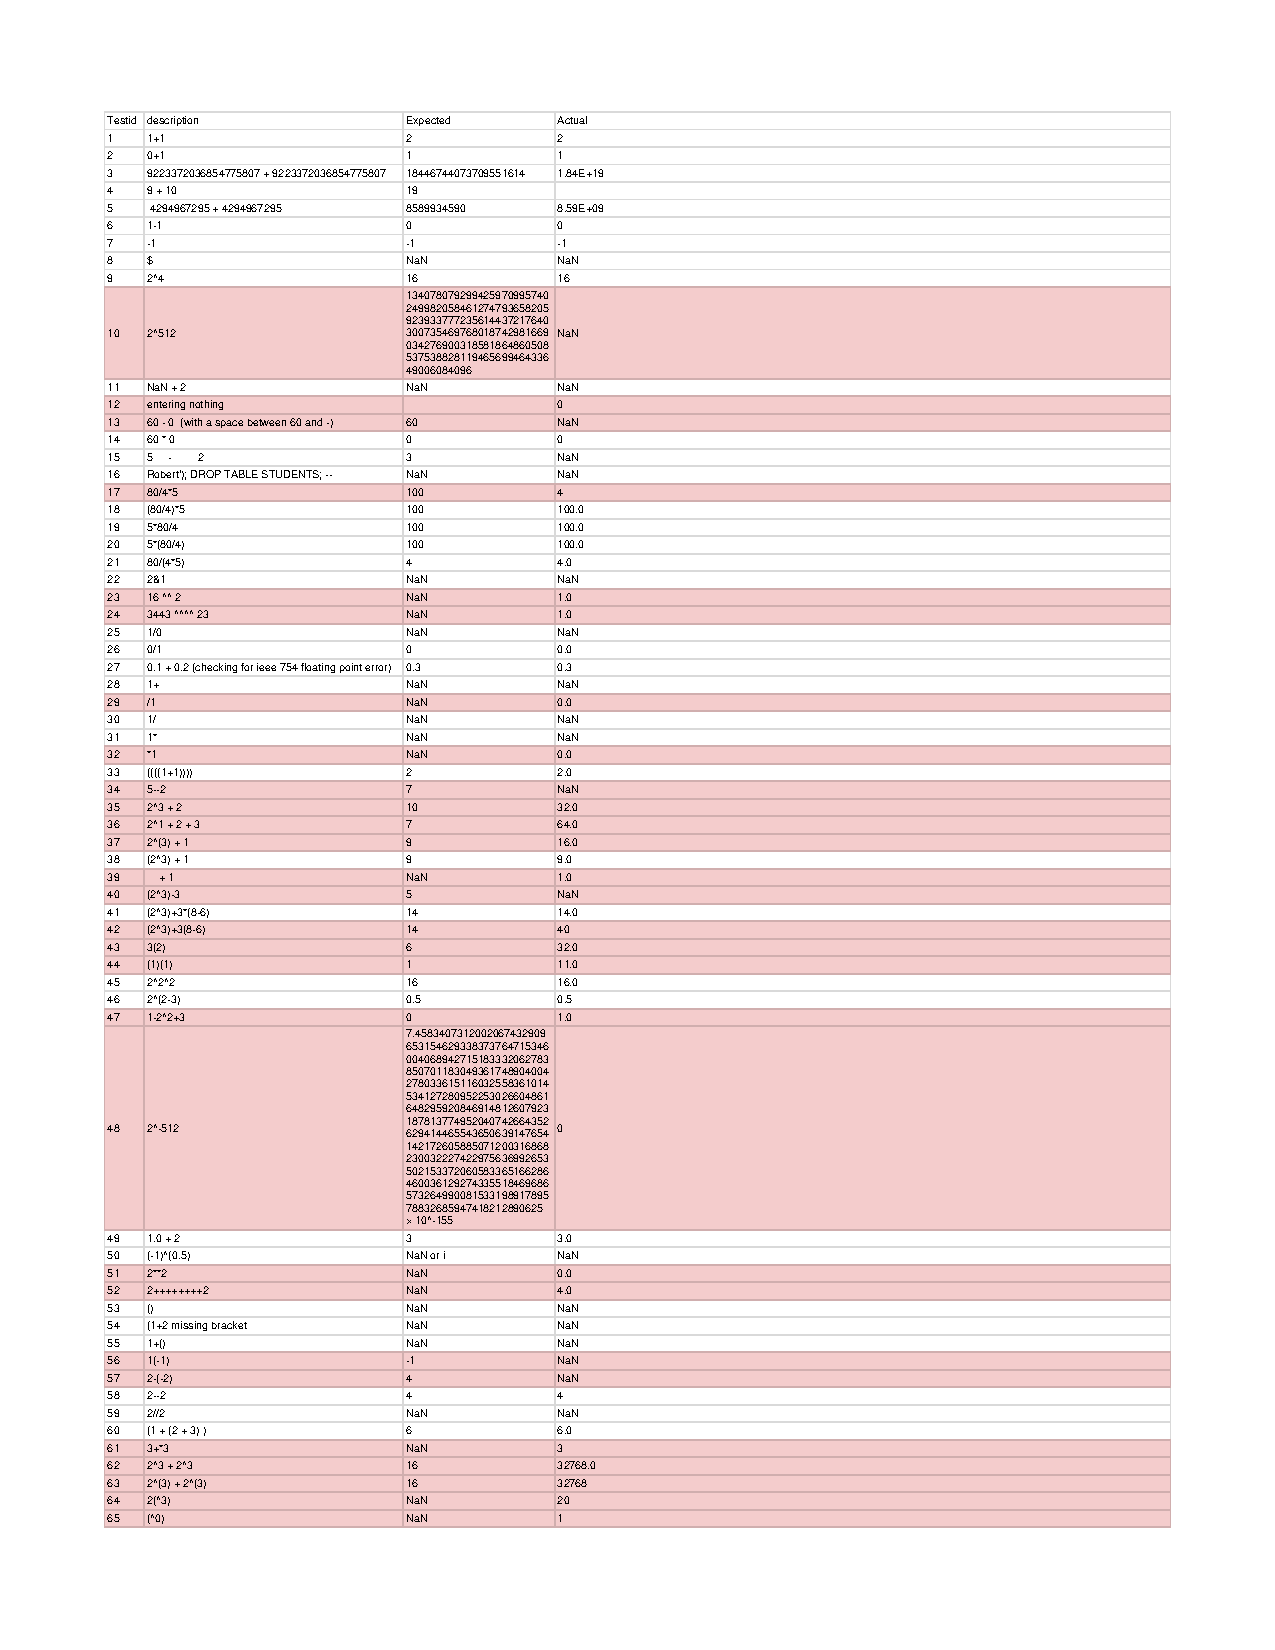
\includepdf[pages=-]{calculatortable.pdf}
\end{document}
